\section{Related Work}

%You should find existing papers, group them into categories based on their approaches, and talk about them: Discuss strengths and weaknesses. In your opinion, which approaches were clever/good? What is the state-of-the-art? Do most people perform the task by hand?
%
%You should have at least 15 references in the related work. Include previous attempts by others at your problem, previous technical methods, or previous learning algorithms. Google Scholar is very useful for this: https://scholar.google.com/ (you can click “cite” and it generates MLA, APA, BibTeX, etc.) You can also try http://www.arxiv-sanity.com/ to search for recent arXiv papers. Try to cite academic publications only (i.e., try to avoid citing blog posts or news articles). Note: arXiv citations are acceptable.

%-------------------------------------------------------------------------

Deep Convolutional Neural Networks have been shown to be very useful for Visual Recognition tasks. AlexNet~\cite{krizhevsky2012imagenet} won the ImageNet Large Scale Visual Recognition Challenge (ILSVRC) in 2012, spurring a lot of interest in using Deep Learning to solve challenging problems. Since then Deep Learning has been used successfully in several fields like Machine Vision, Facial Recognition, Voice Recognition, Natural Language Processing etc.

\begin{figure} 
\centering
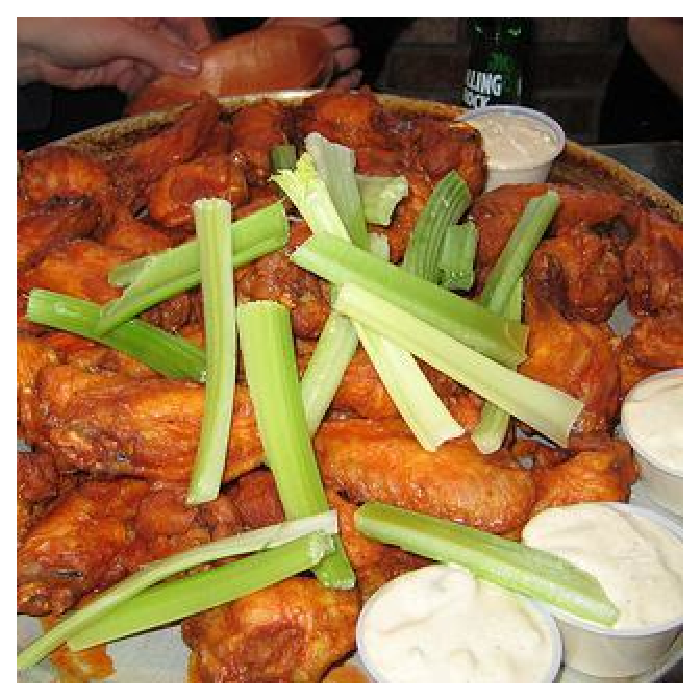
\epsfig{file=Figs4Paper/Buffalo_Wing/f192b38384.eps, height=1.25in, width=1.6in} 
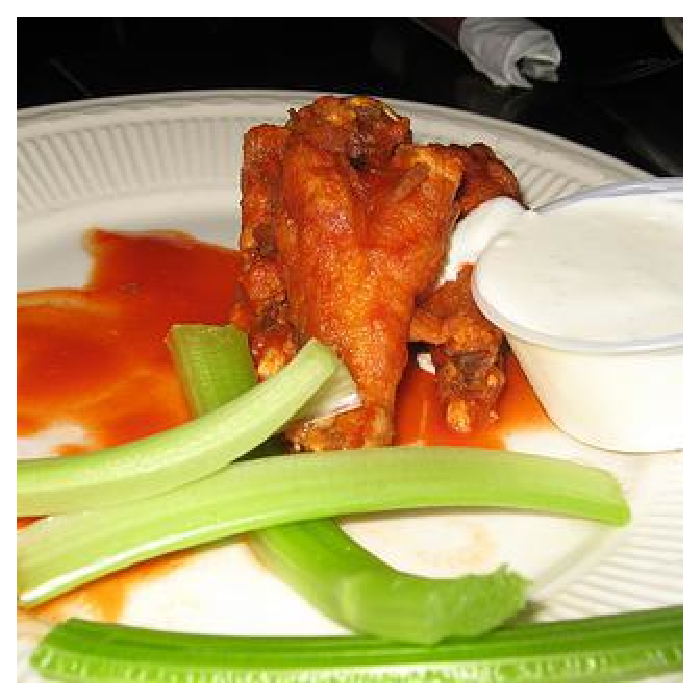
\epsfig{file=Figs4Paper/Buffalo_Wing/e1b0e74a83.eps, height=1.25in, width=1.6in}
\caption{Images of chicken wings dish with celery.}
\label{fig:chickenwingswithcelery}
\end{figure}